\section{Preliminaries}

\noindent
\textbf{Blocks and chains.}
Recall that
the proof-of-work blockchain consists of block headers $B = \left<\textsf{ctr}, \textsf{tx}, s\right>$ each of
which contains a proof-of-work \emph{nonce} $\textsf{ctr}$, a short Merkle Tree~\cite{merkle}
root of transaction
data $\textsf{tx}$, and a pointer $s$ to the previous block in the chain~\cite{backbone}. The value $H(B)$, where
$H$ is a cryptographically secure hash function modelled as a random oracle~\cite{ro}, is used as the $s'$
to include in the next block. Each block must satisfy the proof-of-work equation requiring that
$H(B) \leq T$, where $T$ is the \emph{mining target}. In the \emph{static difficulty model}~\cite{backbone,backbone-new},
$T$ is assumed to be a constant, but in the \emph{variable difficulty model}~\cite{varbackbone}, $T$ varies with
time depending on how much mining power exists on the network. Our final construction will work
in both models, as well as proof-of-stake, but for now let us assume that $T$ is a constant and
that we are working in a proof-of-work setting.

To address blocks within a chain $\chain$, we will use $\chain[i]$ to mean the $i^\text{th}$ (zero-based)
block from the beginning, and $\chain[-i]$ to mean the $i^\text{th}$ (one-based) block from the end.
So $\chain[0]$ indicates the \emph{genesis} block, $\chain[-1]$ is the current tip.
$|\chain|$ denotes the chain length. We use $\chain[i{:}j]$
to denote the subchain starting at the $i^\text{th}$ block (inclusive) and ending at the $j^\text{th}$
block (exclusive).
Omitting $i$ takes the range to the beginning, while
omitting $j$ takes the range to the end.
Similarly, we use $\chain\{A{:}Z\}$ to denote the subchain starting at block $A$
(inclusive) and ending at block $Z$ (exclusive), again allowing for omissions.

In the decentralized setting, each of the honest parties maintaining the blockchain keeps a local
chain $\chain$ which may be different from the others. It is known~\cite{backbone} that these chains
cannot deviate much from each other. In particular, the \emph{Common Prefix} property mandates
that they must all share a long common prefix and can only deviate with forks of length up
to $k \in \mathbb{N}$, a constant determined by the security parameter of the execution.
Formally, if at any round $r_0$ an honest party $P_0$ has adopted a chain $\chain_0$, then
at any round $r_1 > r_0$, any honest party $P_1$ will have adopted a chain $\chain_1$
with the property that $\chain_0[:-k]$ is a prefix of $\chain_1$.
This gives rise to the \emph{safety} property of the ledger: Any transaction that appears
prior to $C[-k]$ is considered confirmed, and it will eventually appear at the same position
in the chains of all honest parties.

The chain of an honest party grows with a certain
rate, which is bounded from below and above with overwhelming probability. This is known as
the \emph{Chain Growth} property (the backbone~\cite{backbone} work contains a proof for the
lower bound; a proof of the upper bound is found in the Appendix).
This gives rise to \emph{liveness}: If a
transaction is submitted to the network, it will eventually appear confirmed to all honest parties,
after at most $\ell \in \mathbb{N}$ blocks have elapsed. These two security parameters $k$ and $\ell$
that govern the evolution of the chain are polynomial in the underlying cryptographic security parameter
$\kappa$, but constant in the execution time.

\noindent
\textbf{Timelock encryption.}
Our construction critically relies on \emph{timelock encryption}.
Timelock encryption allows us to \emph{timelock} a secret so that it can be
unlocked at a prespecified date and time $t$ in the future, but not prior to
that. Timelock encryption consists of two algorithms:

\begin{enumerate}
  \item a \emph{timelock}
        algorithm $\textsf{timelock}(m, t)$, which takes a plaintext message $m$ and a
        timestamp $t$ after which decryption should be possible, and returns a ciphertext $c$
        encrypted for time $t$, and
  \item a \emph{timeunlock} algorithm $\textsf{timeunlock}(c, w)$, which takes a
        ciphertext $c$ encrypted using $\textsf{timelock}$, as well as a witness $w$
        illustrating that indeed time $t$ has passed.
\end{enumerate}

When the time $t$ has elapsed, it becomes easy to compute a \emph{witness} which is
not possible to compute earlier than the target time. At that point, the
\textsf{timeunlock} function can be called with this witness $w$ for time $t$, and it
returns the original message $m$:

\[
  \textsf{timeunlock}(\textsf{timelock}(m, t), w) = m
\]

Prior to time $t$ having elapsed, timelock encryption security mandates that the
ciphertexts corresponding to the encryptions of two plaintexts $m_1$
and $m_2$ should be indistinguishable from one another.

\noindent
\textbf{Witness encryption.}
To construct timelock encryption, it has been proposed~\cite{timelock-bitcoin} to
use \emph{Witness Encryption} (WE). A Witness Encryption scheme is a quite generic
encryption scheme in which a plaintext can be encrypted into a ciphertext that
can be decrypted \emph{only} if a solution to a computational problem is given.
More concretely, the Witness Encryption scheme is parametrized by
an \textsc{NP} language $\mathcal{L}$ (which describes a decision problem)
and an associated relation $\mathcal{R}$ (which verifies a solution to the problem).
The language $\mathcal{L}$ is a set of \emph{problem instances} $x$ (the inputs
for which the problem answer is \emph{yes}). For each instance
$x \in \mathcal{L}$, there exists a witness $w$ such that $x\mathcal{R}w$ holds. For
non-instances $x \not\in \mathcal{L}$, no such witness exists. The relation $\mathcal{R}$
is polynomially computable.

A witness encryption scheme, parametrized by an \textsc{NP} language given by relation $\mathcal{R}$
consists of two algorithms:

\begin{enumerate}
  \item an \emph{encryption} algorithm $\textsc{WE.Enc}_\mathcal{R}(m, x)$, which takes a plaintext
        $m$ and a problem instance $x$ and returns a ciphertext $c$ encrypted for this problem instance,
        and
  \item a \emph{decryption} algorithm $\textsc{WE.Dec}_\mathcal{R}(c, w)$, which takes a ciphertext
        $c$ and a witness $w$ and returns the decrypted plaintext $m$ as long as $x \mathcal{R} w$.
\end{enumerate}

The \emph{correctness} of the witness encryption requires that, whenever $x \mathcal{R} w$, it holds
that $\textsc{WE.Dec}_\mathcal{R}(\textsc{WE.Enc}_\mathcal{R}(m, x), w) = m$. On the other hand, the \emph{security}
of the scheme mandates that an adversary
given $c = \textsc{WE.Enc}_\mathcal{R}(m, x)$
can extract information about $m$
only if they can also produce
(through a helper \emph{extractor} machine)
a valid witness $w$ such that $x \mathcal{R} w$, except with negligible probability.
Hence, a correct and secure witness encryption scheme allows a party to decrypt a ciphertext encrypted
with a problem instance \emph{if and only if} the party can solve the problem instance by providing a
witness.

To construct timelock encryption using witness encryption, the problem statement asks for the
existence of a series of blockchain work nonces that solve the proof-of-work equation (or a series
of correctly signed proof-of-stake blocks with the appropriate chain length), as illustrated
in Figure~\ref{fig.blockchain-timelock}.

The instantiation of timelock encryption using witness encryption
begins by identifying the chain tip $B$. The timelock time $t$
is expressed in chain time: We ask that a certain number of blocks must have been mined on top of $B$
in order for the secret to become decryptable. The witness encryption \textsc{NP} language contains
the integers $t \in \mathbb{N}$ indicating that there exists a block with additional block height
$t$ descending from the known block $B$. The witness consists of a series of nonces $\textsf{ctr}_i$
and transaction root hashes $\textsf{tx}_i$ such that
$B_0 = B$ and
$B_i = \left<\textsf{ctr}_i, \textsf{tx}_i, H(B_{i-1})\right>$
and $H(B_i) \leq T$,
where $i$ ranges from $1$ to $t$. Therefore, the timelock function $\textsf{timelock}(m, t)$ is defined
as $\textsf{WE.Enc}_\mathcal{R}(m, x)$ where $\mathcal{R}$ corresponds to the relation checking the
validity of the blockchain and $x$ corresponds to the number of blocks $t$ as well as the current
chain tip $B$. The unlock function $\textsf{timeunlock}(c, w)$ is defined as
$\textsf{WE.Dec}_\mathcal{R}(c, w)$ under the same relation $\mathcal{R}$ where $w$ consists of
the sequence of $\textsf{ctr}_i$ and $\textsf{tx}_i$. For the security proof of instantiating timelock
encryption using witness encryption applied on a blockchain, consult Liu et al.~\cite{timelock-bitcoin}.

\begin{figure}[ht]
    \caption{A timelock implemented using the moderately hard \textsc{NP} language of blockchain discovery.
             Here, the problem instance $x = (B, t)$ requests $t = 7$ blocks on top of $B$. The witness
             consists of the block headers produced sequentially on top of $B$, irrespective of any
             temporary forks that might have occurred.}
    \centering
    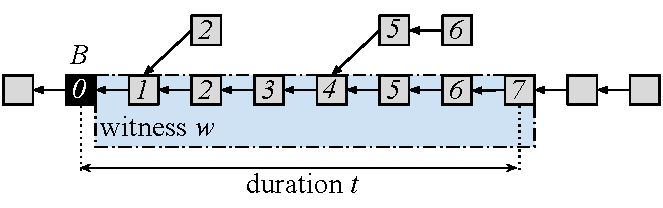
\includegraphics[width=0.8 \columnwidth,keepaspectratio]{figures/blockchain-timelock.pdf}
    \label{fig.blockchain-timelock}
\end{figure}

Let us observe what the outcome of encrypting secrets in this manner is. Whenever a secret is encrypted
for block time $t$ following block $B$, the secret remains hidden until time $t$ has arrived.
The secret cannot be decrypted prior to that time, because decrypting it would require the decrypting party
to produce (through an extractor) a witness $w$ which is a blockchain of height $t$ extending $B$. However,
due to the \emph{Common Prefix} property of the blockchain, no adversary can do that much sooner than the
honest parties converge to that height. Furthermore, the \emph{chain growth} rate is bounded both \emph{above} (see
Appendix for a short proof of this)
and \emph{below}~\cite{backbone} by a certain \emph{velocity}, and so, while we do not know its exact growth rate, we can give
a reasonable estimate of how quickly and slowly it will grow (with overwhelming probability).
When sufficient time has elapsed, the miners will have produced a witness that anyone can use to decrypt the
secret. The result is that no one can know the secret prior to the desired block height, but everyone will
know it afterwards. Because the adversary can have a chain that is leading by up to $k$ blocks, she has
a short advantage in decrypting the secret slightly ahead of the honest parties. In that sense, the
secret begins \emph{leaking} to the adversary at block time $t - k$. This will require us to establish
certain time bounds in our construction.
Note here that no validity is ensured in $\textsf{tx}_i$, but the common prefix property of blockchains
makes this unnecessary.

Our security proof will hinge on the fact that the blockchain has the \emph{common prefix} property: If
an adversary can decrypt the witness encrypted ciphertext \emph{much} earlier than the honest parties,
then she will need to have produced a chain which significantly deviates from the honest parties' chain,
but this is improbable.

The witnesses to these problem instances can grow linearly together with the blockchain. To reduce witness
size, a (zero knowledge) proof of knowledge such as a zk-SNARK~\cite{EPRINT:BCTV13} can be used.
In this case, instead of
witness encrypting against a decryptor who
``knows a witness consisting of a list of chain headers that satisfy the blockchain properties,''
one can instead witness encrypt against a decryptor who
``knows a witness consisting of a zero-knowledge proof of knowledge attesting to the knowledge of chain headers
that satisfy the blockchain properties.'' This composition of witness encryption and zero-knowledge proofs
allows the witnesses presented to the blockchain to become constant size~\cite{timelock-bitcoin}.

Contrary to timelock schemes that require the interested party to devote compute power to decrypt the secret
over time, the scheme using blockchain witnesses allows any party (who can remain offline and have limited compute
power) to take advantage of the scheme.

\noindent
\textbf{Variable difficulty.}
In the variable difficulty model, the target $T$ is adjusted based on how the chain evolves.
Concretely, the chain is split into \emph{epochs} of constant block length $m$ each. At the end of each
epoch, the timestamp at the end of the chain is noted and the mining target is adjusted with the
aim of keeping the expected block production rate constant.
The
way $T$ is adjusted is algorithmically determined, and it is important that it follows certain
rules. While we will not articulate the exact rules, we remark that the new value $T'$ must fall
within a range $\tau T, \frac{1}{\tau} T$, where $\tau \in (0, 1)$ (for example, Bitcoin sets
$\tau = \frac{1}{4}$). This critical condition is necessary to avoid certain attacks~\cite{bahack}.

\noindent
\textbf{Proof-of-stake.}
Contrary to proof-of-work blockchains, a proof-of-stake chain progresses in \emph{slots}
(prefixed time durations) during which
parties can create blocks or remain silent.
As in proof-of-work, each block header $B_i$ consists of $\left<\textsf{tx}_i, s_i\right>$, but now
does not include a $\textsf{ctr}_i$.
The blocks created at each slot are accompanied by a
signature $\sigma_i$ created by a designated leader for the slot.
A proof $\pi_i$ illustrating the designated leader is the rightful one
is also broadcast together with the block.
The probability that a party becomes a leader at a given slot is roughly
proportional to the stake they hold within the system.
These proofs of leadership are different depending on the system and can
be the random outcome of a multiparty computation, as in the \emph{Ouroboros}~\cite{ouroboros} system,
or a verifiable random function~\cite{FOCS:MicRabVad99} evaluated on this randomness, as in
the \emph{Ouroboros Praos}~\cite{praos} construction.
In the first system,
each slot is allocated to precisely one party, and the production of no blocks, or two competing blocks in the
same slot, indicates adversarial behavior. In the second system, it is possible that a slot is allocated
to multiple honest parties, or no parties at all. These details do not affect our scheme, as long as the following
property is maintained: For any $2k$ consecutive slots, at least $k+1$ slots are allocated to an honest
party. Additionally, we will assume that the common prefix property holds here, too.

As in proof-of-work, the chain is split into epochs.
At the end of each epoch, a multiparty computation is performed to determine
the randomness value for the next epoch based on the stake distribution during the current epoch.
Different systems use different MPCs. Our only requirement is that these MPCs provide some
evidence $u_e$ that the randomness for epoch $e$ is $\rho_e$. This evidence must be
polynomially checkable in retrospect. This requirement is satisfied in proof-of-stake blockchains,
as it is this evidence that allows new nodes to bootstrap correctly~\cite{ouroboros-genesis}.
